\chapter{Synthetic Training Images}\label{chap:synthetic}

Training the DNNs that are used by WCA applications for physical assembly tasks
requires thousands of labeled images.
Capturing and labeling these images requires substantial effort.
Bounding boxes must be drawn around the region of each image that
contains the object being assembled.  The bounding box must then be
labeled with the step of the assembly process that is depicted in the
image.  Collecting and labeling a training set of images is a major
barrier to entry for anyone who wants to develop a WCA application for
a new task.
For example, this effort took over 50 person hours for the Ikea Cart application
described in Section~\ref{sec:ikea_cart}.
This task had 17 different states.
This time-consuming and labor-intensive
aspect of WCA is the biggest bottleneck to its widespread adoption.

Previous papers have proposed the use of synthetically generated
images for training sets.  In this approach, pre-labeling is done by
construction~\cite{synthetic_data, DBLP:journals/corr/abs-1809-10790,
  photo2, real_background1, real_background2, real_background3,
  dwibedi}.  Since programs that generate synthetic images have
information about the objects that are visible and their locations,
there is no need for manual input of this information.  In addition,
synthetic images of objects can easily be rendered in a wide variety
of different lighting conditions and environments.  In contrast,
capturing real images of objects in a variety of conditions requires
the images of the object to be captured in every such environment.
Overall, the use of synthetic data may save considerable manual
effort.

This chapter presents our experience training DNNs for WCA applications for
three assembly tasks, using synthetic training images.

\section{Meccano Erector Kit}

In this section, we ask how well synthetic images work for creating a WCA
application for assembling a Meccano Erector Kit.
We use the following procedure to answer this
question.  We first generate a set of synthetic (pre-labeled) images
using the Unity Perception package~\cite{unity}.
Unity is a video game engine that includes 3D graphics rendering capabilities
and CAD tools.
The Perception package was created by Unity to enable the creation of object
detectors from CAD models instead of real images that had to be labeled with
bounding boxes.
This package can create thousands of images, and it will render the subassembly
in a different location in each one.
It outputs a label file with each image, that contains the coordinates that the
subassembly in that image was rendered at.
This eliminates the need to manually label images with bounding boxes.

After generating the synthetic images with Unity, we train
computer vision models on this data.  Next, we  collect and manually
label a set of real images for the same task, and then train computer
vision models on this data.  Finally, we compare the accuracy of these
two families of models on a held-out test set of real images.  Our
results show that models created with a training set size of 75,000
synthetic images perform slightly better than models created with
roughly 15,000 real images.
However, this ordering is reversed when fewer synthetic images are used for
training.

The Meccano Kit assembles into a model bike.
The fully assembled model is depicted in Figure~\ref{fig:full_bike}.
It is made from over 50 parts.
However, this work will only separate the bike into three subassemblies.
The fine-grained classifiers we trained for this kit had 5 output labels.
Three of the labels were for the individual subassemblies, and the remaining two
were for the steps required to put the subassemblies together.

\begin{figure}
  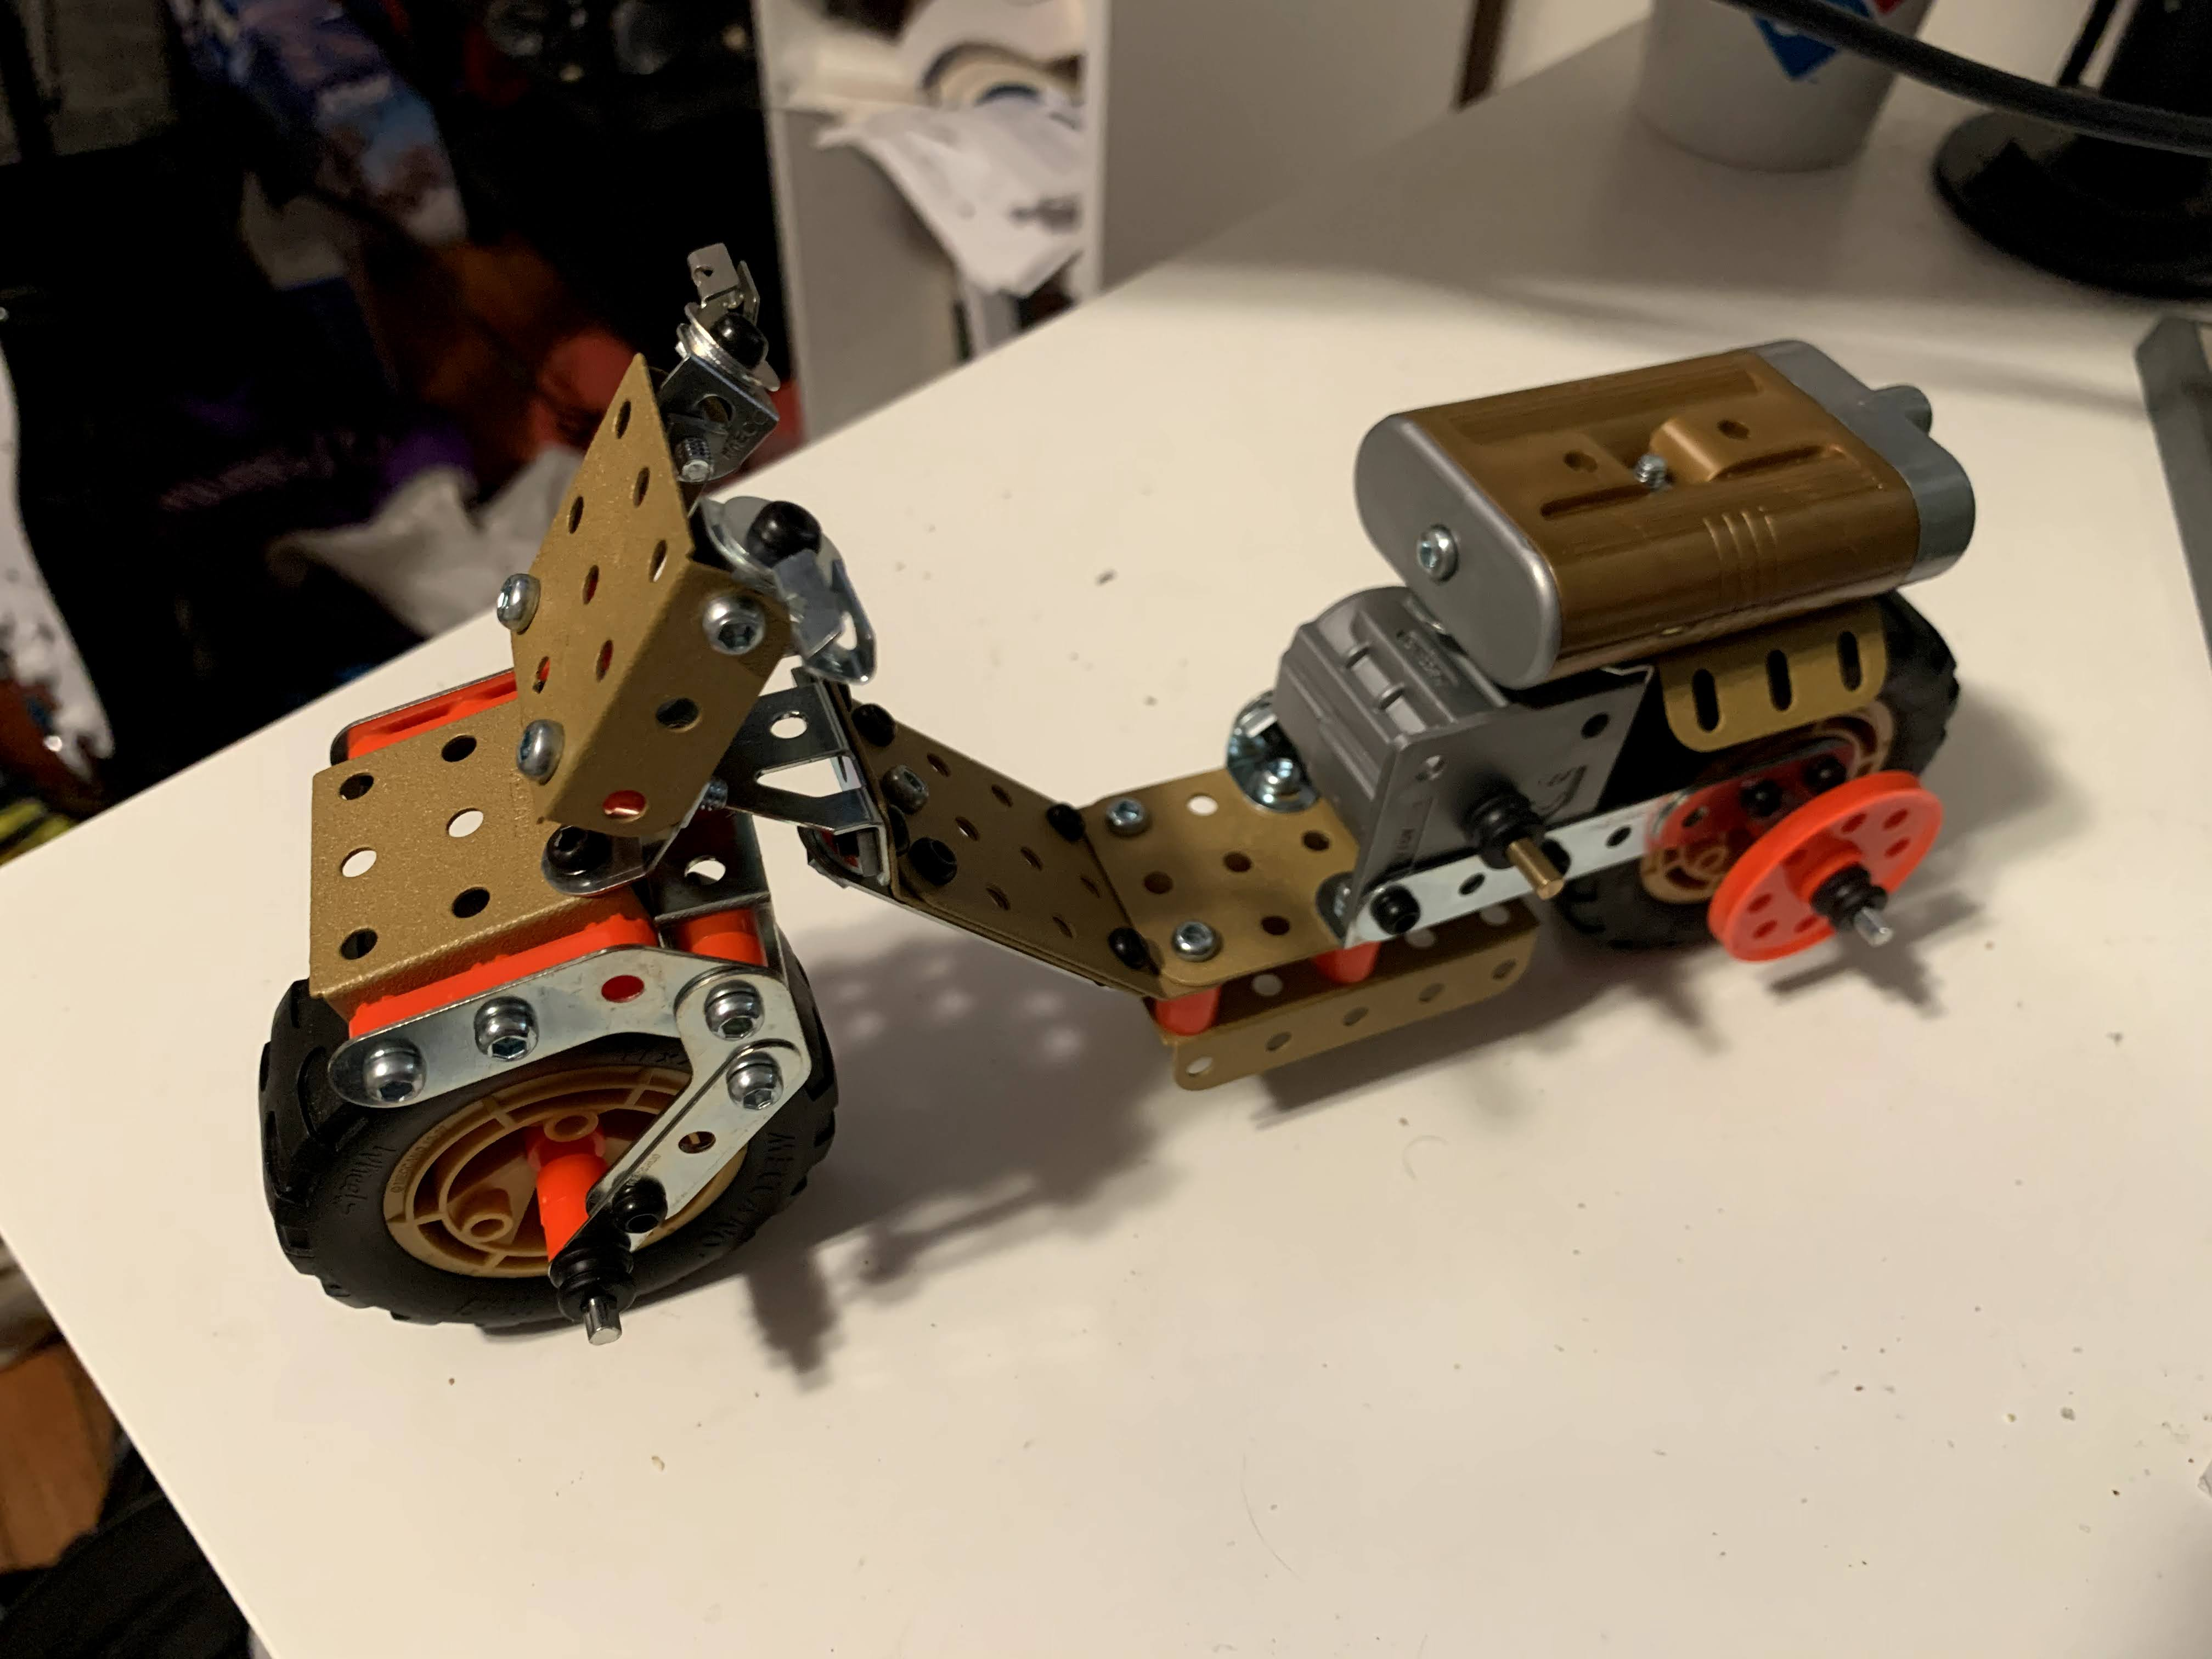
\includegraphics[width=\columnwidth]{figures/synthetic/full_bike.jpg}
  \caption{
    The fully assembled model bike.
  }\label{fig:full_bike}
\end{figure}

\subsection{Generating Data}

We found a computer-aided design (CAD) model for the Meccano kit on the
community website
GrabCAD\footnote{\url{https://grabcad.com/library/meccano-9550-002-1}}.
This CAD model appears to have been created to replicate the physical Meccano
pieces, rather than being the same model that was used to manufacture the
pieces.
In particular, we noticed a number of differences between the CAD model and the
actual Meccano parts.
We selected textures for each part of the model, trying to match the
appearance of the physical object as closely as possible.
We generated synthetic images using the Unity Perception Package~\cite{unity}.
The default setup for this package fills the background of the images that are
generated with objects that the network should learn to ignore.
Figure~\ref{fig:perception_default} shows an image generated using this default
setup.

\begin{figure}
  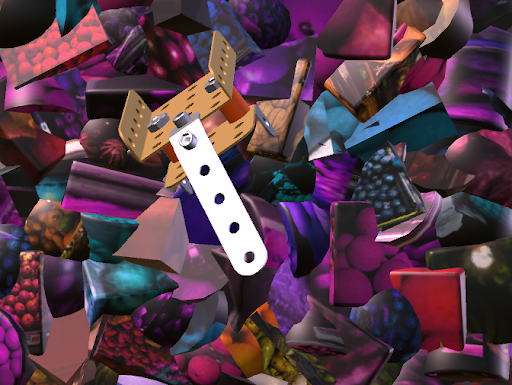
\includegraphics[width=\columnwidth]{figures/synthetic/perception_default.png}
  \caption{
    A synthetic image showing part of the bike model. The background is filled
    with distractor objects that the network should learn not to identify.
  }\label{fig:perception_default}
\end{figure}

The Unity Perception Package allowed us to make some of the individual parts of
the CAD model invisible.
This enabled us to generate synthetic images for each step of the task.
For a given step, we specified the parts of the subassembly that were visible.
We were then able to generate thousands of synthetic images for this step.
The perception package generated a label file for each synthetic image, that
specified the coordinates of a bounding box around the subassembly and a label
name corresponding to the step of the task that was shown in the image.

We trained a Faster R-CNN object detector using this data.
The Unity package creates a file with bounding box and label information, and
we converted this to the format used by the TensorFlow Object Detection API.
The perception package drew bounding boxes tightly around the objects.
We added padding to these bounding boxes, to make them more like our hand-drawn
labels (which also had some padding).
Figure~\ref{fig:padding} shows bounding boxes with and without padding.
Training the object detector on images with padding resulted in the object
detector returning bounding boxes with some padding.
This resulted in higher intersection over union scores when evaluating our
object detectors on test data with hand-drawn labels.

\begin{figure}
  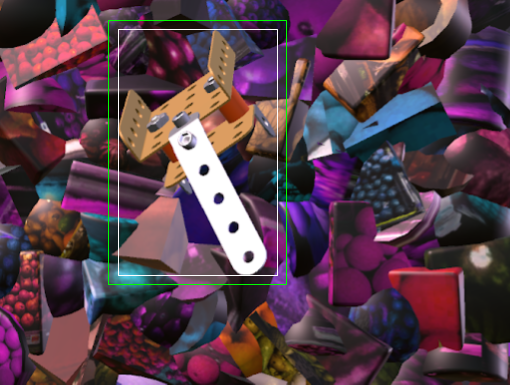
\includegraphics[width=\columnwidth]{figures/synthetic/padding.png}
  \caption{
    The white bounding box has no padding.
    The Unity perception package uses bounding boxes without padding.
    The green bounding box has padding.
    Our dataset uses bounding boxes with padding.
  }\label{fig:padding}
\end{figure}

Unfortunately the training process for this model did not converge.
We attempted to fix this issue by removing the background objects from the
image, and then we tried to make the objects look like they were sitting on a
wooden floor.
We accomplished this by placing the object at the bottom of the 3D scene in
Unity and texturing the floor of the scene with an image of wood from Adobe's
collection of stock images.
Figure~\ref{fig:wood_floor} shows one of these images.
The Faster R-CNN model trained on this data converged; however, it performed
poorly.
One issue that we noticed was the object detector mistakenly detected lines
in the wood floor as being a model bike assembly.
Figure~\ref{fig:false_positive} shows an example of such an erroneous detection.

\begin{figure}
  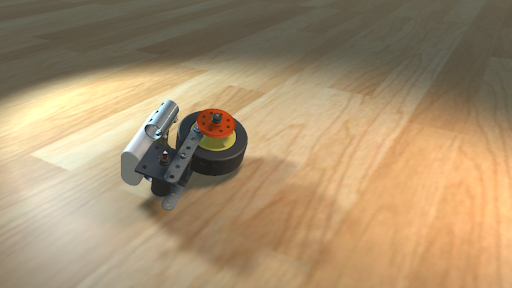
\includegraphics[width=\columnwidth]{figures/synthetic/wood_floor.png}
  \caption{
    Our first attempt at making our synthetic images look more realistic.
    This image is meant to look like an object sitting on a wood floor.
  }\label{fig:wood_floor}
\end{figure}

\begin{figure}
  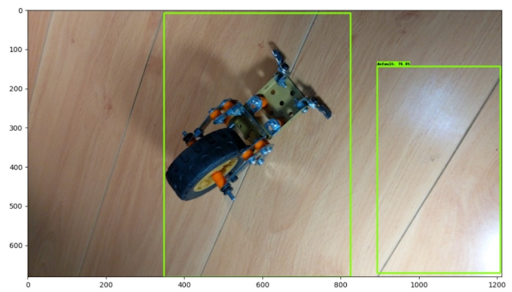
\includegraphics[width=\columnwidth]{figures/synthetic/false_positive.png}
  \caption{
    A case where our model incorrectly detected a line in the floor as an
    object of interest.
    The green bounding boxes are regions of the image in which the model
    detected an object.
  }\label{fig:false_positive}
\end{figure}

We were able to correct this issue by using additional background textures and
randomizing the lighting in the scene and the position of the camera.
We have posted our code\footnote{\url{https://github.com/exiaohuaz/data-gen}}.
Figure~\ref{fig:good_data} shows some examples of this data.
Figure~\ref{fig:adobe_backgrounds} shows some of the background images that we
used.

\begin{figure}
  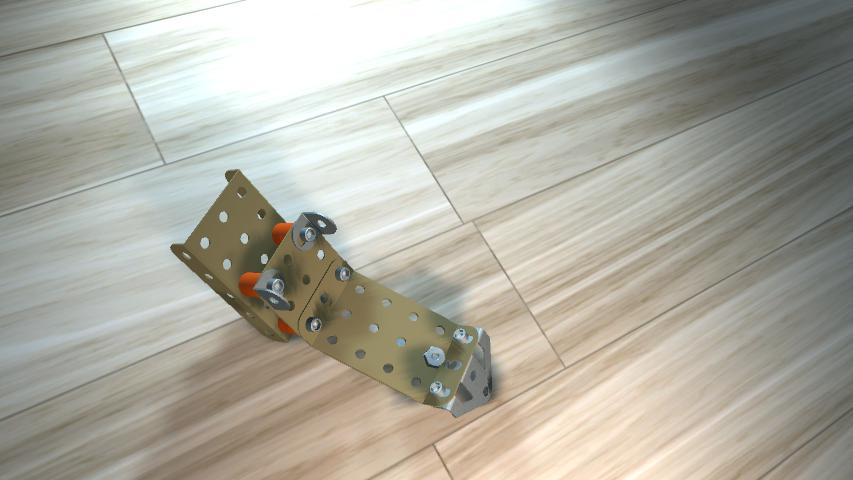
\includegraphics[width=0.5\columnwidth]{figures/synthetic/floor1.jpg}
  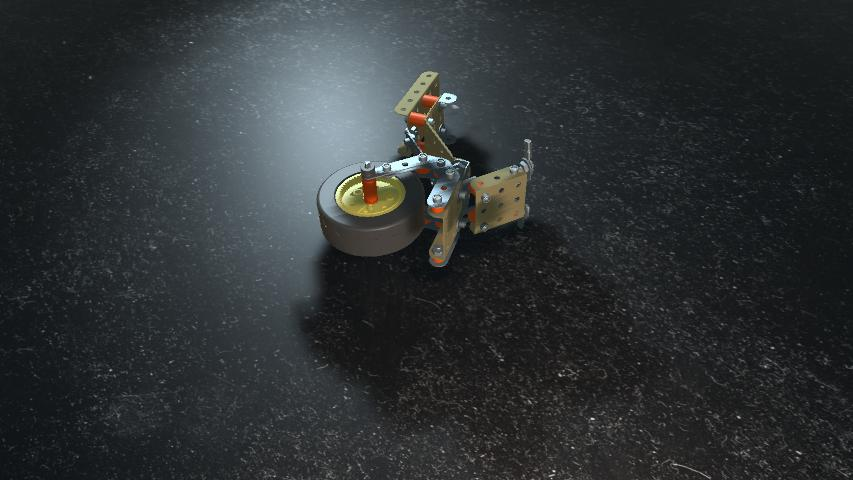
\includegraphics[width=0.5\columnwidth]{figures/synthetic/floor2.jpg}
  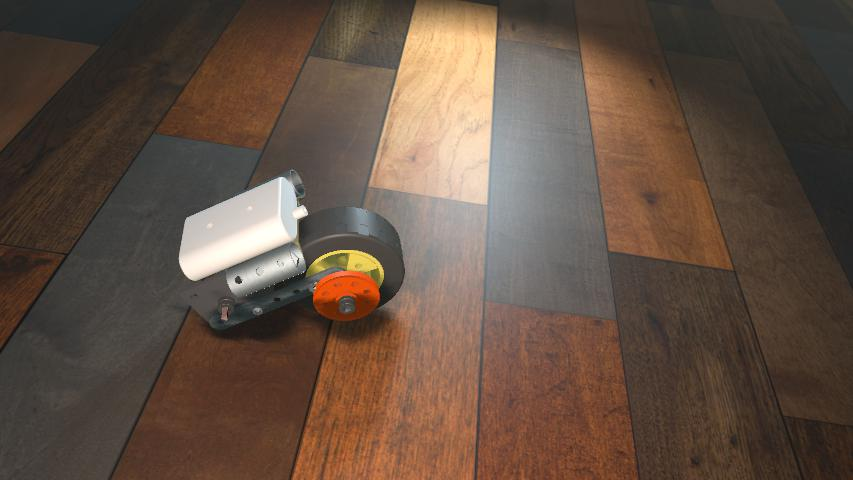
\includegraphics[width=0.5\columnwidth]{figures/synthetic/floor3.jpg}
  \caption{
    Synthetically generated images from our final set. The models trained on
    this data performed well.
  }\label{fig:good_data}
\end{figure}

\begin{figure}
  
\includegraphics[width=0.33\columnwidth]{figures/adobe_stock/concrete.jpg}
  
\includegraphics[width=0.33\columnwidth]{figures/adobe_stock/wood1.jpg}
  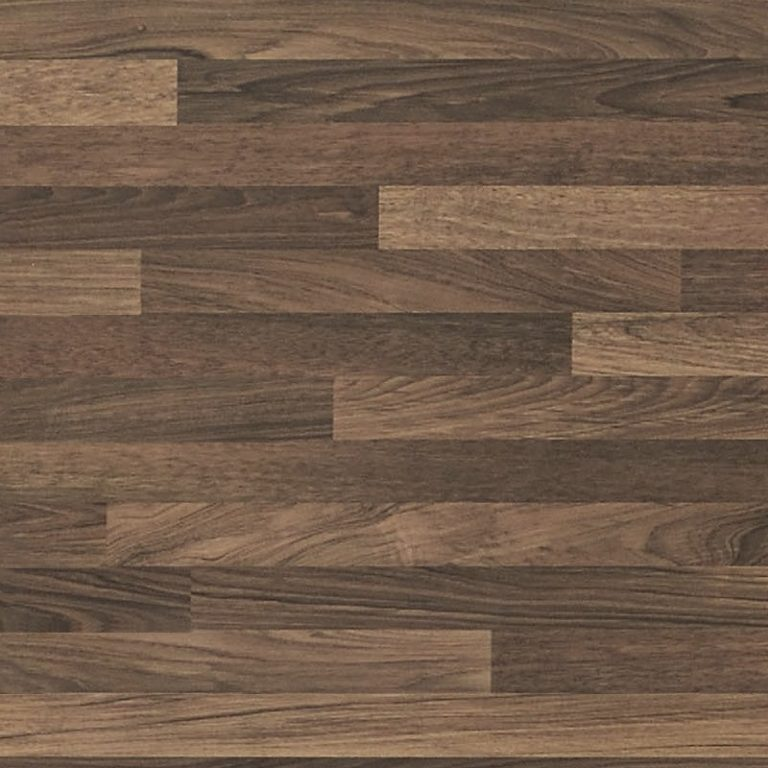
\includegraphics[width=0.33\columnwidth]{figures/adobe_stock/wood2.jpg}
  \caption{
    Examples Images from Adobe Stock that we used as background textures.
  }\label{fig:adobe_backgrounds}
\end{figure}

After training the Faster R-CNN object detector to find the location of a
subassembly, we trained a Fast MPN-COV classifier to determine the step of the
task that is shown in the region found by the Faster R-CNN model.
Henceforth, we will use the term model pair to describe a Faster R-CNN object
detector and a Fast MPN-COV classifier created using the same training set.

\subsection{Results}

We evaluated our model pipelines based on accuracy, which is the percentage of
images in the test set that were classified correctly.
This is equivalent to both top-1 accuracy and micro F1 score.
Classification tasks are typically evaluated using top-K accuracy, which
looks at the K labels that the model outputs as being most likely.
If any of the K labels are correct, the output is considered correct.
The value of K is varied based on what seems reasonable for the specific task.
Setting K to 5 makes sense for a dataset like Imagenet, with 1000 different
labels.
However, all of our models were trained on labels for a single subassembly.
Each subassembly was built in under 10 steps, so our models had fewer than 10
output labels.
In addition, a WCA application can only give a user one instruction at a time.
Our classifiers must reliably output the one correct label in order to be
useful.
We thus chose top-1 accuracy as our evaluation metric, rather than selecting a
larger value of K.

All of our training and testing data relates to
uncluttered environments with good lighting.
We assume that a human
using a WCA application can correct environmental issues to reduce
classification complexity.  For example, the user can increase the
amount of light shining on an assembly, or remove clutter from the
background.
Assuming near-optimal environmental conditions for a WCA assembly
task is thus reasonable.

We trained one model pair on real data that was manually labeled with
bounding boxes and class labels (15,477 images).
The remaining model pairs were trained on synthetic data sets of varying size
(12,000, 25,000, 50,000 and 75,000 images).
The labels for these images were generated by Unity.
We compared the accuracy of these model pairs.

Our test set consists of 4490 real images that are not included in any
training set.  Table~\ref{tab:meccano_accuracy} presents our results.  We
observe that the model trained on real data performs better than the
models trained on synthetic datasets with 12,000, 25,000, and 50,000
images.  However, this relationship is reversed for a model trained on
75,000 synthetic images.
Somewhere between 50,000 and 75,000 images
lies the cross-over point at which the increased number of synthetic
images more than compensates for their lower realism.
Changing the quality of the synthetic data, changing the quality of the real
data, or changing the amount of real data could change the location of the
cross-over point.

\begin{table}
\begin{tabular}{|l||l|l|}
\hline
  Dataset Type & Training Set Size & Accuracy\\
  \hline
  \hline
  Synthetic & 12,500 & 69.6\%\\
  Synthetic & 25,000 & 79\%\\
  Synthetic & 50,000 & 84.1\%\\
  Synthetic & 75,000 & 89\%\\
  \hline
  Real & 15,477 & 84.5\%\\
\hline
\end{tabular}
  \caption{
    Classification results for our model pairs for the Meccano kit.
    Accuracy is the percentage of our 4490 test images that the pipeline of
    models classified correctly.
  }\label{tab:meccano_accuracy}
\end{table}

\section{Toy Plane}

The next kit we generated synthetic images for was a toy plane that was made up
of 3D printed plastic parts.
This kit contained six unique parts, and required four steps to assemble.
Figure~\ref{fig:assembled_plane} shows what the physical kit looks like when it
is fully assembled.
Figure~\ref{fig:plane_parts} shows the CAD models for the individual parts while
Figure~\ref{fig:plane_steps} shows the CAD models for the assembly steps.

\begin{figure}
  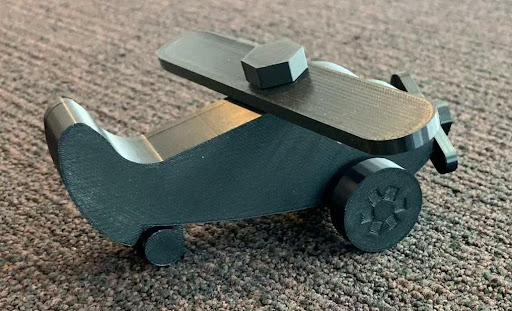
\includegraphics[width=\columnwidth]{figures/synthetic/toy_plane.jpg}
  \caption{
    The fully assembled model plane kit. All parts are 3D printed plastic.
  }\label{fig:assembled_plane}
\end{figure}

\begin{figure}
  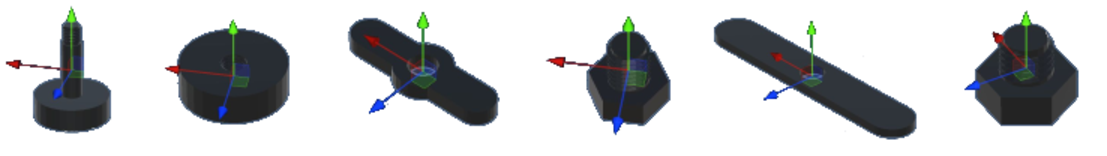
\includegraphics[width=\columnwidth]{figures/synthetic/plane_parts.pdf}
  \caption{
    CAD models for the individual model plane parts.
  }\label{fig:plane_parts}
\end{figure}

\begin{figure}
  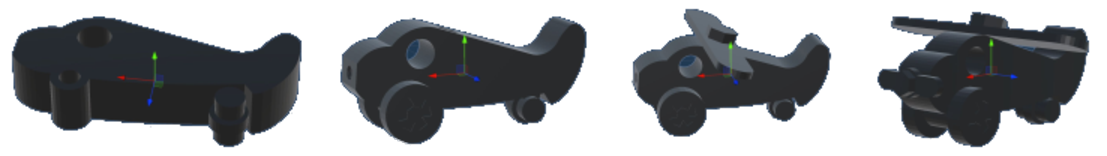
\includegraphics[width=\columnwidth]{figures/synthetic/plane_steps.pdf}
  \caption{
    CAD models for the model plane assembly steps.
  }\label{fig:plane_steps}
\end{figure}

We downloaded the CAD file for this kit from the community website
Cults~\footnote{\url{https://cults3d.com/en/3d-model/game/toy-plane-assembled-by-bolts-and-nuts}},
and then 3D printed the kit using this file.
We will refer to objects generated from a CAD model that we have access to as
being ``born digitally.''

We captured real images of the 3D printed parts using a smartphone camera,
labeled these images with CVAT, and trained a model pair on this data.
Next, we generated synthetic training images using the Unity Perception Package.
Figure~\ref{fig:plane_train} contains examples of these images.
Afterwards, we trained model pairs on sets of these synthetic images, with
varying sizes.

All of our model pairs for the toy plane were tested on a set of 14,996 real
images that was separate from any of the images used during training.
The results of these tests are shown in Table~\ref{tab:plane_accuracy}.
All of our model pairs that were trained on synthetic images performed better
than the model pair trained on 39,643 real images.
This was different than what we observed with the Meccano kit.
The model pair trained on 75,000 synthetic training images of the Meccano
kit outperformed the model pair trained on real images of the Meccano kit.
However, the model pair trained on real images of the Meccano kit outperformed
all of the model pairs trained on fewer than 75,000 synthetic images.
One possible reason that synthetic data was more effective for the toy plane
than the Meccano kit is that training on synthetic data might be more effective
for objects with simpler surfaces.
The toy plane is made out of simple plastic, while the Meccano kit is made out
of more complex metals.

As we observed with the Meccano kit, the accuracy of our models increased with
the size of the training set.
However, the increases in accuracy were less dramatic than the increases in
accuracy for the Meccano kit, because the model pair trained on the smallest
dataset achieved a high accuracy.

\begin{figure}
  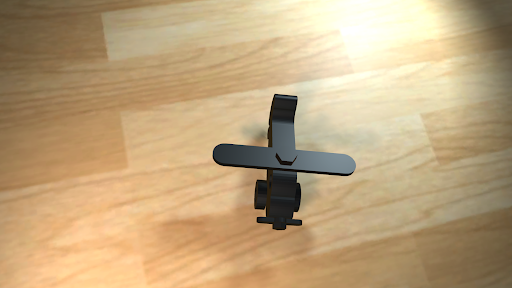
\includegraphics[width=0.5\columnwidth]{figures/synthetic/plane_train1.png}
  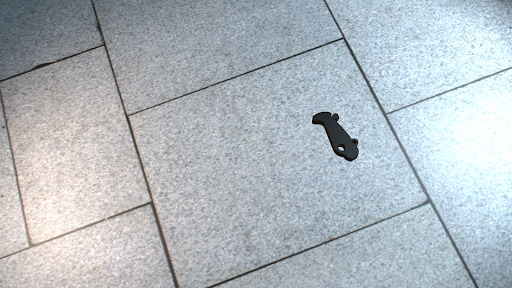
\includegraphics[width=0.5\columnwidth]{figures/synthetic/plane_train2.png}
  \caption{
    Synthetically generated training images for the toy plane kit.
  }\label{fig:plane_train}
\end{figure}

\begin{table}
\begin{tabular}{|l||l|l|}
\hline
  Dataset Type & Training Set Size & Accuracy\\
  \hline
  \hline
  Synthetic & 12,500 & 87.7\%\\
  Synthetic & 25,000 & 89.3\%\\
  Synthetic & 50,000 & 90.0\%\\
  \hline
  Real & 39,643 & 76\%\\
\hline
\end{tabular}
  \caption{
    Classification results for model pairs trained on data for the toy plane.
    Accuracy is the percentage of our 14,996 test images that the pipeline of
    models classified correctly.
  }\label{tab:plane_accuracy}
\end{table}

\section{Phone Sanitizer}

The final kit we generated synthetic training data for was a sanitizer for a
smartphone.
This kit contained a large metal base and several plastic parts.
Figure~\ref{fig:full_sanitizer} shows the kit fully assembled.
The kit contained four unique parts, and there were five steps required to
assemble it.
Thus there were 9 output labels from the fine-grained classifier.

\begin{figure}
  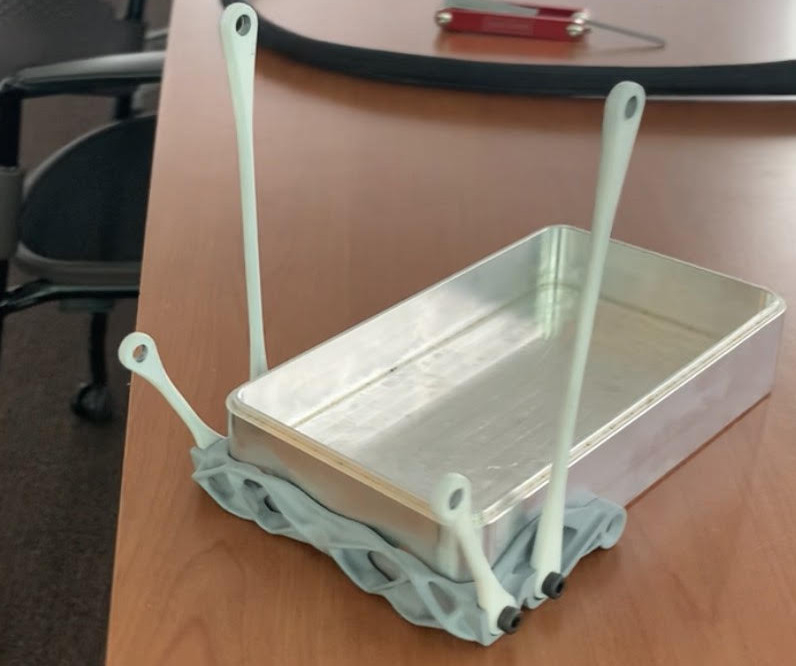
\includegraphics[width=\columnwidth]{figures/synthetic/full_sanitizer.jpg}
  \caption{
    The fully assembled Phone Sanitizer.
  }\label{fig:full_sanitizer}
\end{figure}

As with the toy plane, this kit was born digitally, and we had access to the
CAD files that the parts were manufactured from.
We generated synthetic training images for the sanitizer using the Unity
Perception~\cite{unity} package and Autodesk A3D~\cite{Wang_2022_CVPR}.
Figure~\ref{fig:sanitizer_unity} shows images from the training set that was
generated using Unity while Figure~\ref{fig:sanitizer_a3d}
shows images from the training set that was generated using
A3D.
Both sets of data were used to train model pairs that were then evaluated on
60,129 real images.
As with our other synthetic datasets, we trained model pairs on different sized
datasets.
The results from these evaluations are presented in
Table~\ref{tab:sanitizer_accuracy}.
The results from the models trained on images from A3D were noticeably better
than the model pairs trained on the Unity data.
We again observed that model pairs trained on larger datasets performed better.

\begin{figure}
  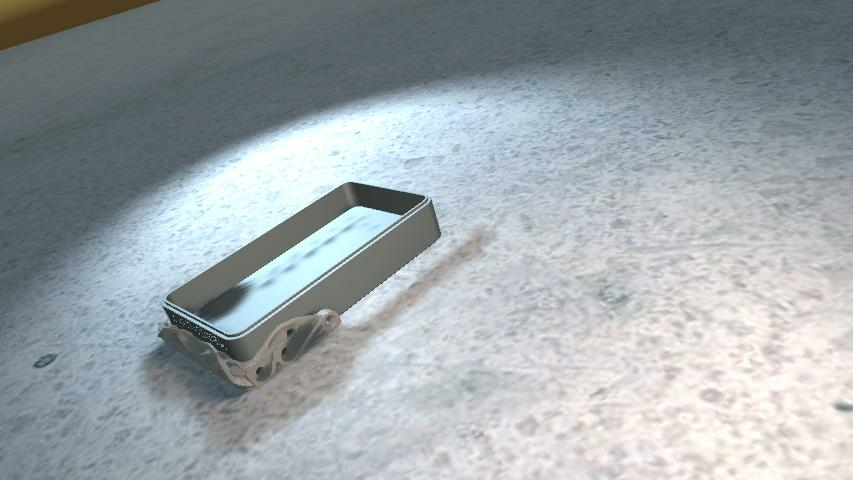
\includegraphics[width=0.5\columnwidth]{figures/sanitizer/unity1.png}
  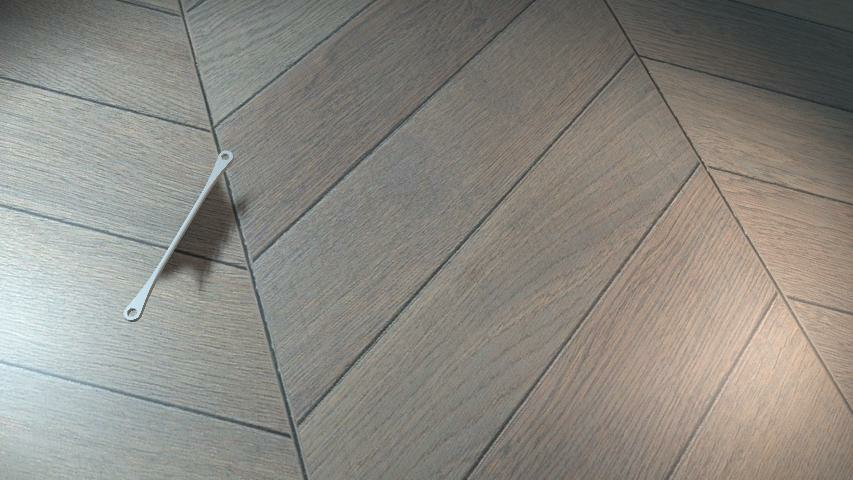
\includegraphics[width=0.5\columnwidth]{figures/sanitizer/unity2.png}
  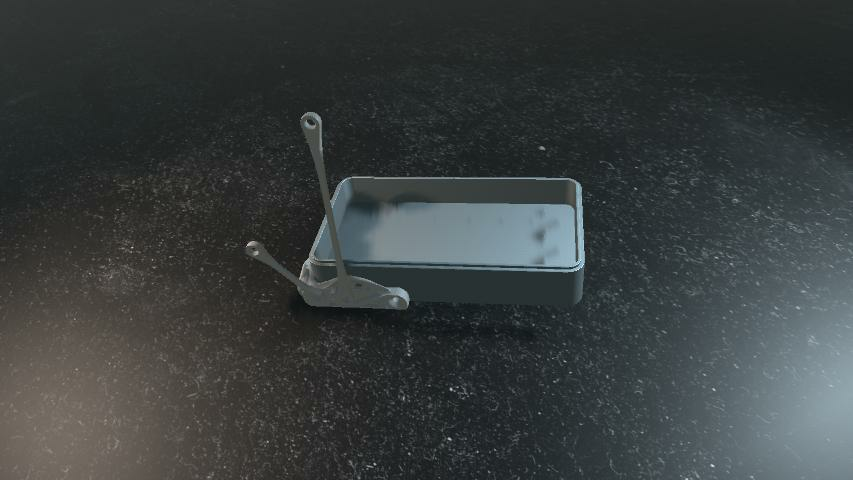
\includegraphics[width=0.5\columnwidth]{figures/sanitizer/unity3.png}
  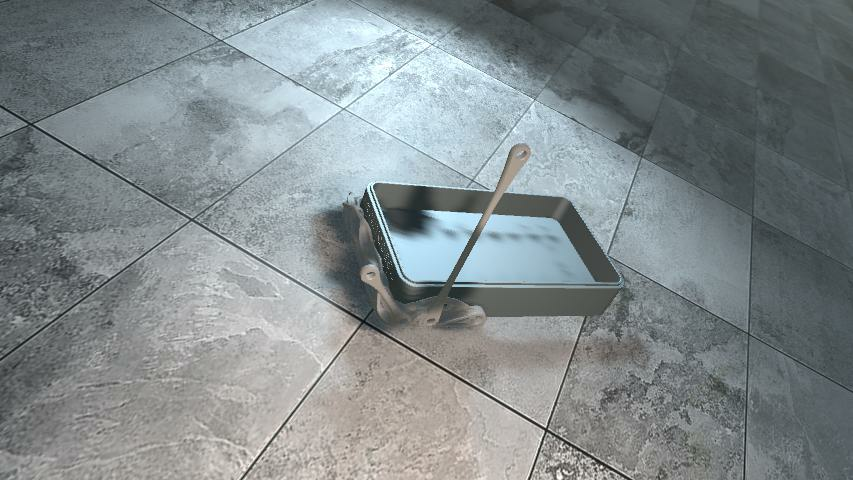
\includegraphics[width=0.5\columnwidth]{figures/sanitizer/unity4.png}
  \caption{
    Synthetic training images for the phone sanitizer task, generated using the
    Unity Perception Package.
  }\label{fig:sanitizer_unity}
\end{figure}

\begin{figure}
  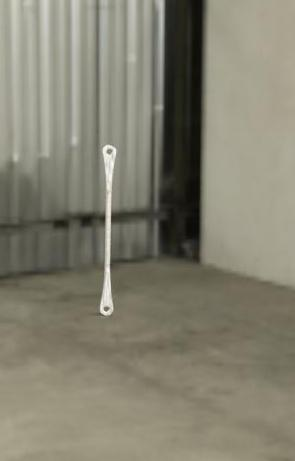
\includegraphics[width=0.5\columnwidth]{figures/sanitizer/a3d1.jpg}
  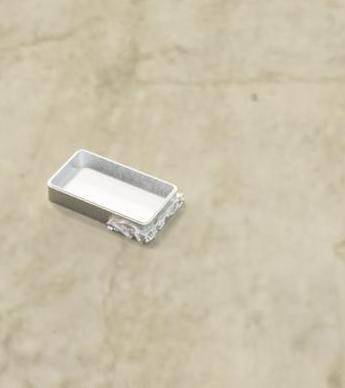
\includegraphics[width=0.5\columnwidth]{figures/sanitizer/a3d2.jpg}
  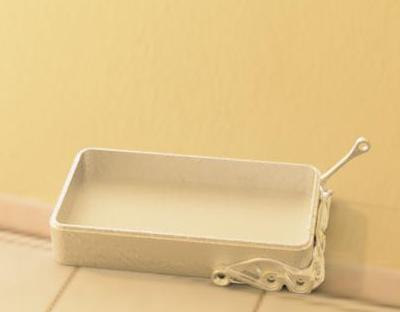
\includegraphics[width=0.5\columnwidth]{figures/sanitizer/a3d3.jpg}
  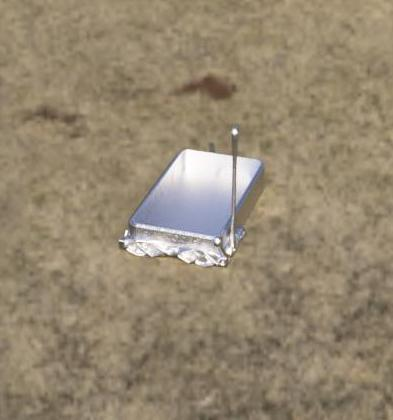
\includegraphics[width=0.5\columnwidth]{figures/sanitizer/a3d4.jpg}
  \caption{
    Synthetic training images for the phone sanitizer task, generated using
    Autodesk A3D.
  }\label{fig:sanitizer_a3d}
\end{figure}

\begin{table}
\begin{tabular}{|l||l|l|}
  \hline
  & Unity & A3D\\
  \hline
  \hline
  12,500 & 75\% & 89.6\% \\
  \hline
  25,000 & 81.2\% & 91.6\%\\
  \hline
  50,000 & 85\% & 92.9\%\\
  \hline
\end{tabular}
  \caption{
    Classification results for model pairs trained on synthetically generated
    images of the phone sanitizer.
    The top row of the table indicates the software used to create the dataset.
    The left column of the table indicates the size of the training set.
    The values in the table are the percentage of our 60,129 test images that
    the pipeline of models classified correctly.
  }\label{tab:sanitizer_accuracy}
\end{table}

The textures of the sanitizer parts in the A3D images were more realistic than
the textures of the parts in the Unity images.
In particular, the metal surfaces in the A3D images reflect light more
accurately than the metal surfaces in the Unity images.
We hypothesized that the realistic textures were responsible for A3D images
resulting in models that were more accurate than the Unity images.
To verify this hypothesis, we generated a set of images using A3D that used much
simpler textures.
Figure~\ref{fig:sanitizer_a3d_simple} shows examples of these images.
We created three different sized training sets using these images.
Table~\ref{tab:sanitizer_accuracy_simple_textures} lists the accuracies of
models trained on these sets, tested on the test set of real images.
The accuracy was considerably lower than the models trained on our original A3D
dataset, with the same number of images.
This supports our hypothesis that realistic textures were responsible for
the superior performance of the models trained on the A3D images, when
compared with model pairs trained on Unity images.

The model pair trained on 12,500 images was 0.5\% more accurate than the model
pair trained on 25,000 images.
This is a very small difference in performance, but it is unexpected.
One possible explanation for this difference is that the 25,000 image dataset
contained a set of particularly problematic images that were not in the 12,500
image dataset.
The images might have been problematic due to lighting or orientation of the
subassembly.
These problematic images might have eliminated any benefit that the larger
dataset offered.
The model pair trained on 50,000 images was more accurate than either of the
model pairs that were trained on smaller datasets.

\begin{figure}
  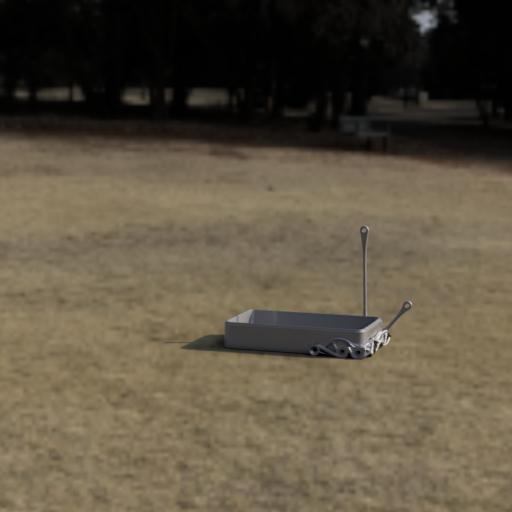
\includegraphics[width=0.33\columnwidth]{figures/synthetic/simple1.jpg}
  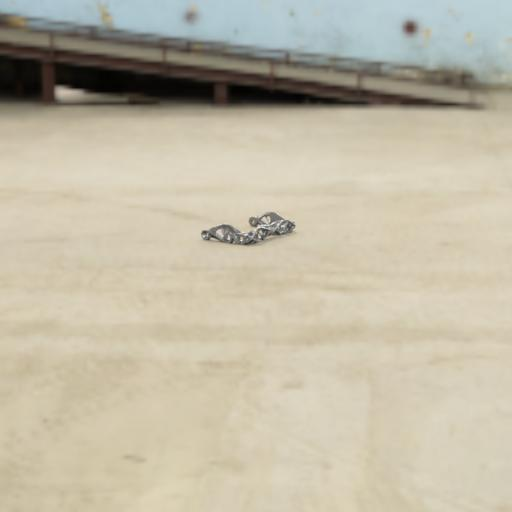
\includegraphics[width=0.33\columnwidth]{figures/synthetic/simple2.jpg}
  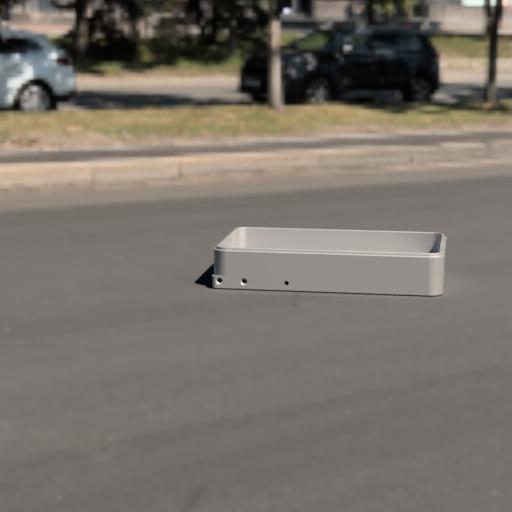
\includegraphics[width=0.33\columnwidth]{figures/synthetic/simple3.jpg}
  \caption{
    Images generated using A3D with simple object textures.
  }\label{fig:sanitizer_a3d_simple}
\end{figure}

\begin{table}
\begin{tabular}{|l|l|}
  \hline
  Dataset Size & Accuracy\\
  \hline
  \hline
  12,500 & 77.3\%\\
  \hline
  25,000 & 76.8\%\\
  \hline
  50,000 & 78.84\%\\
  \hline
\end{tabular}
  \caption{
    Classification results for model pairs trained on simple texture synthetic
    images of the phone sanitizer from A3D.
    Accuracy is the percentage of our 60,129 test images that the pipeline of
    models classified correctly.
  }\label{tab:sanitizer_accuracy_simple_textures}
\end{table}

\section{Discussion}

Capturing and labeling training images for WCA applications is a time
consuming process.  Using synthetic images is less labor-intensive,
and would simplify development of WCA applications.  We have achieved
promising results with this approach for three different assembly tasks.
These results offer the tantalizing promise that
using synthetic data might eliminate the need to manually capture and label
images in order to develop WCA applications for assembly tasks.

\citet{Wang_2022_CVPR} note several ways that A3D could be improved to make
images look better.
We believe that all of these proposed changes, especially the improvements to
camera positioning, could result in better training data for the types of
computer vision models that we use.
In addition, software tools liked Autodesk A3D and the Unity Perception package
can be made easier to use.
A developer must create individual CAD files for each step of a task.
For example, if the models must recognize a certain kit with a screw
inserted and without that screw inserted, the developer must create a CAD file
showing the kit before this screw is removed and another CAD file showing the
kit after this screw is removed.
Open Workflow Editor allows a developer to specify a task using a flowchart.
Adding the ability to specify the parts of a CAD model that get inserted or
removed during a task step would make it easier to develop
WCA applications for kits that are born digitally.
In addition, integrating tools for automatic Assembly sequence
planning~\cite{subassembly_identification} into these programs would improve WCA
application development.

After a developer has generated synthetic images, the number of manual steps
required to achieve a working WCA application is still very high.
Autodesk A3D and the Unity Perception package both output annotations in
different formats.
The developer must convert these into the format used by the TensorFlow Object
Detection API, and create another copy in the format used by the Fast MPN-COV
implementation.
Afterwards, the developer must start training object detectors and fine-grained
images classifiers needed by the application.
The developer must then create a flowchart in Open Workflow Editor that
specifies the task instructions and the models that should be used at each step
of the task.
We are actively working to simplify this process.
